% Chapter Template

\chapter{Feed forward optimum pitch control.} % Main chapter title

\label{Chapter3} % Change X to a consecutive number; for referencing this chapter elsewhere, use \ref{ChapterX}


%----------------------------------------------------------------------------------------
%	SECTION 1
%----------------------------------------------------------------------------------------

\section{Introduction} \label{section3-1}
As discussed in Section \ref{section1-2}, the closed loop control system of a typical utility scale wind turbine manipulates generator torque and collective blade pitch in order to control the power generation and rotor speed of the turbine. At low and medium wind speeds the blade pitch remains fixed at 0\degree while generator torque is manipulated to achieve the rotor speed that maximizes electricity generation. At high wind speeds the collective blade pitch is manipulated to manage loading on the wind turbine as well as to maintain constant rotor speed and power generation. For a given wind speed there is a desired rotor speed ($\Omega_{Rotor}$), collective blade pitch ($\theta$), and generator torque ($T_{Gen}$). Figure \ref{fig3-1} shows these desired values for the NREL 5-MW turbine. If the wind remained constant the control system of the NREL 5-MW turbine would bring $\Omega_{Rotor}, \theta, and T_{Gen}$ to the values shown in figure \ref{fig3-1} and maintain those desired conditions. However, since wind speed often fluctuates (as shown in figure \ref{fig3-2}) and utility scale turbines are large mechanical devices that are unable to instantaneously adjust to changes in wind speed, turbines are frequently chasing the desired conditions instead of operating at the desired conditions.

\begin{figure}[htb]
	\centering
		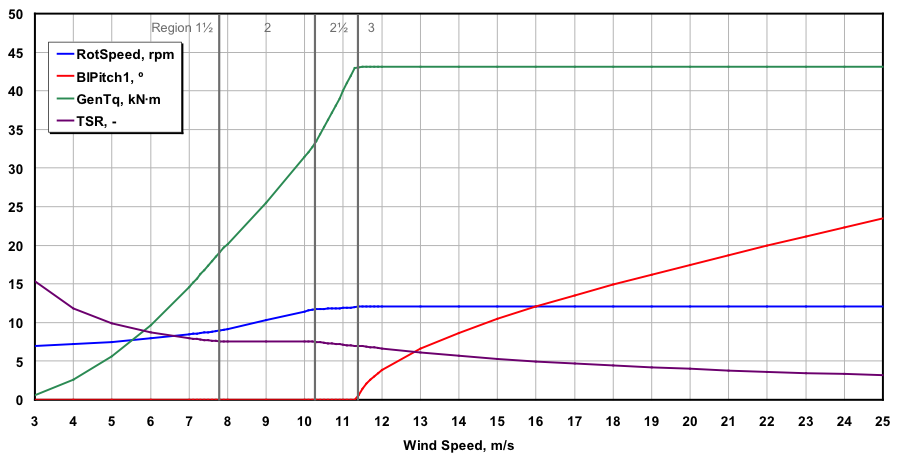
\includegraphics[width=\linewidth]{Figures/ch2Figures/fig2-1.png}
		
	\caption{Steady state behavior of the NREL 5-MW.\cite{jonkman2009}}
	\label{fig3-1}
\end{figure}

\begin{figure}[htb]
	\centering
		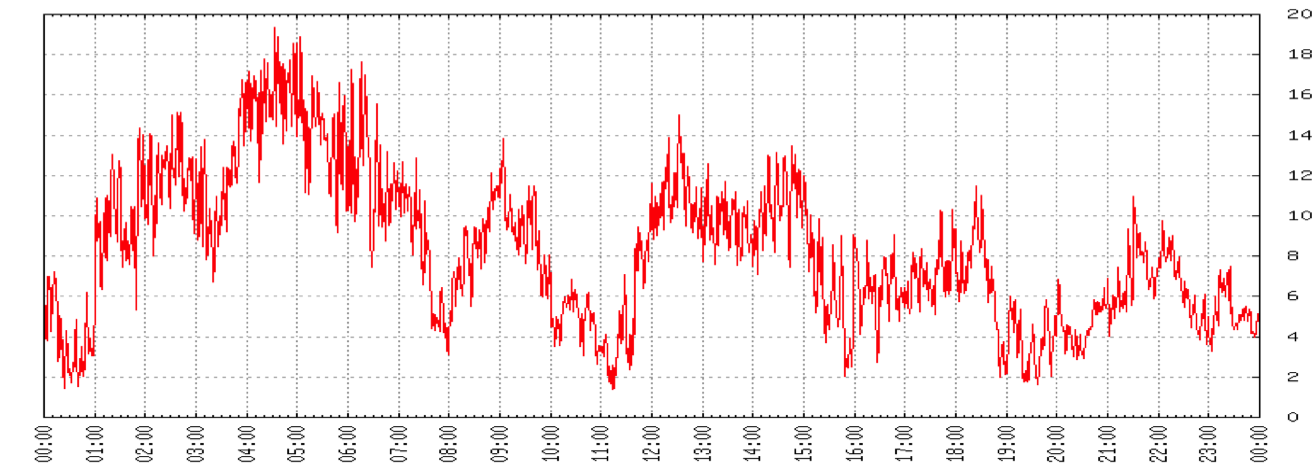
\includegraphics[width=\linewidth]{Figures/ch3Figures/fig3-2.png}
		
	\caption{An example of wind speed fluctuations over 24 hours.\cite{NWTC2013}}
	\label{fig3-2}
\end{figure}

Figures  \ref{fig3-3} and  \ref{fig3-4} illustrate the transient response of the NREL 5-MW turbine when subjected to sudden changes in wind speed. In both cases FAST has been used to model a NREL 5-MW turbine with the baseline controller defined in \cite{jonkman2009}. Figure \ref{fig3-3} illustrates turbine behavior in region 2, wind speeds between 7.8 m/s and 10.3 m/s, while Figure \ref{fig3-4} illustrates turbine behavior in region 3, wind speeds between 11.4 m/s and 25 m/s.  Each figure shows wind speed, ``Actual'' and ``Optimal'' power, generator torque, and blade pitch. ``Actual'' power is the power generated by the turbine. ``Optimal'' power is the desired steady state power generation for the current wind speed (based on the NREL 5-MW power curve shown in Figure \ref{fig1-6}). Generator torque and blade pitch are the two actuators used to control turbine performance. 

In Figure \ref{fig3-3} the turbine is subjected to a uniform incoming wind that changes between 8 m/s and 10 m/s every 20 seconds. These wind speeds are in region 2, where optimal power production corresponds to the maximum aerodynamic efficiency of the turbine. Note that the turbine takes approximately 20 seconds to reach optimal generation after each change in wind speed. This corresponds to a reduction in efficiency.  The optimal power curve generates 0.6\% more power (15.6 kW on average) than the actual power curve. In this case turbine performance is regulated entirely by torque control. The turbine blades remain at 0$^{\circ}$ pitch. 

\begin{figure}[htbp]
	\centering
		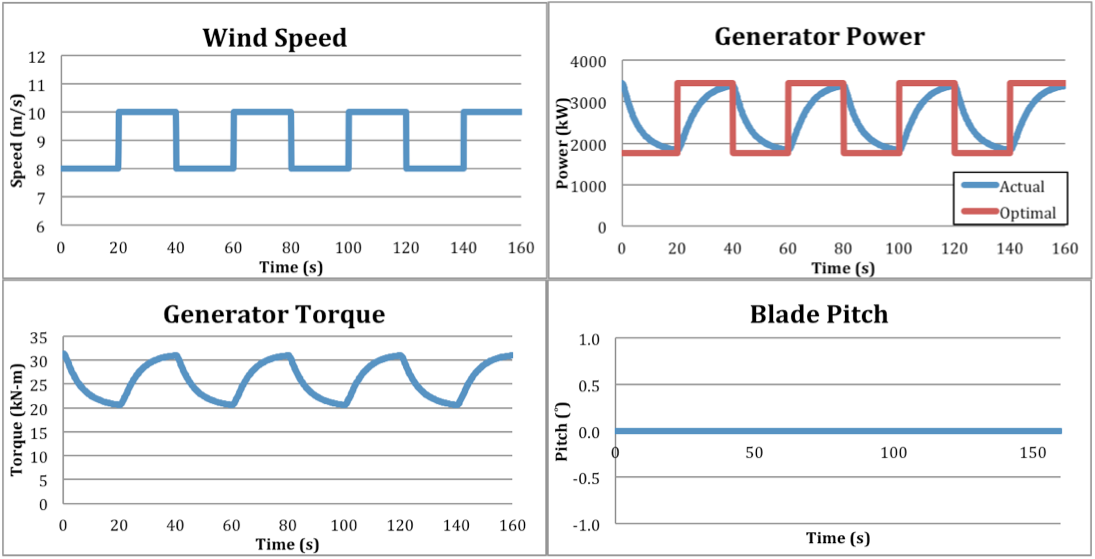
\includegraphics[width=\linewidth]{Figures/ch3Figures/fig3-3.png}
		
	\caption{NREL 5-MW response to wind speed fluctuations in control region 2.}
	\label{fig3-3}
\end{figure}

In Figure \ref{fig3-4} the turbine is subjected to a uniform incoming wind that changes between 16 m/s and 18 m/s every 40 seconds. These wind speeds are in region 3, where optimal power production is the rated power of the turbine, 5 MW. After each change in wind speed the turbine experiences both spikes and dips in power production.  The largest fluctuations in power occur in the first 10 seconds after a change in wind speed. After 25 seconds the generated power is nearly constant at 5 MW.  In this case turbine performance is regulated by both torque control and pitch control. 

\begin{figure}[htbp]
	\centering
		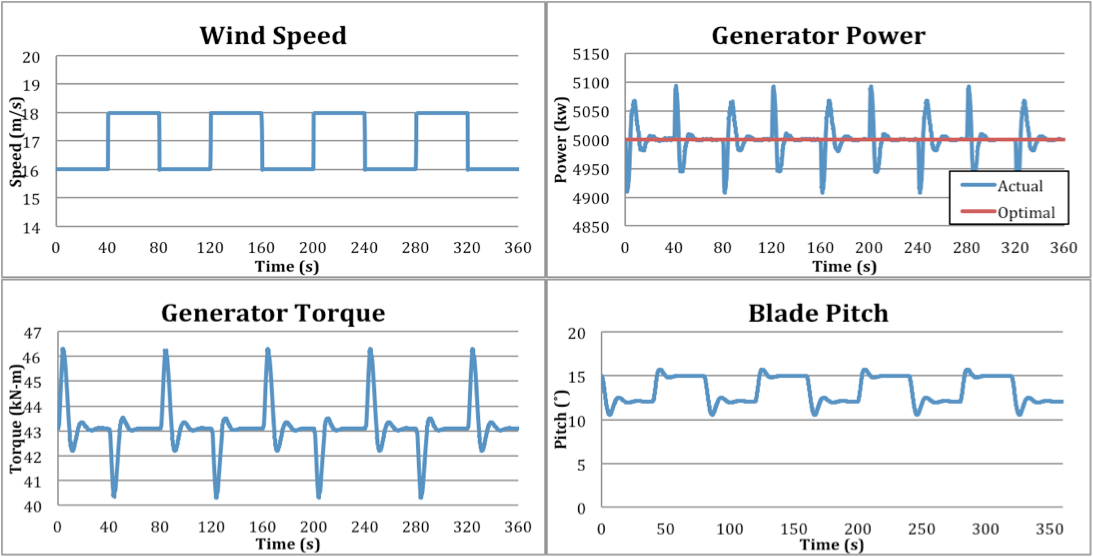
\includegraphics[width=\linewidth]{Figures/ch3Figures/fig3-4.png}
		
	\caption{NREL 5-MW response to wind speed fluctuations in control region 3.}
	\label{fig3-4}
\end{figure}

The previous figures show that wind turbines respond reactively to changes in wind speed. However, several researchers have shown that turbine performance can be improved if a turbine is able to pre-emptively react to changes in wind speed before they occur. Ozdemir, Seiler, and Balas showed that perfect preview knowledge of incoming wind speed could be used to increase power production or decrease gearbox loads by improving generator torque control in region 2 operation. The authors used state space optimal control techniques to control generator torque based on incoming fluctuations in wind speed. In some of their simulations they were able to achieve increases in power generation of 6\% or decreases in gerabox loading of 30\%.\cite{ozdemir2013} Dunne, Pao, Wright, Jonkman, Kelley, and Simley have shown that perfect preview knowledge of incoming wind speed fluctuations could also be used reduce turbine loads by improving pitch control in region 3 operation. The authors examined three methods of feed forward pitch control based on wind speed preview information: non-causal series expansion, preview control, and optimized FIR filter methods. The authors simulated the response of the feed forward controllers to both turbulent wind and sudden gusts. Each of the feed forward controllers were capeable of reducing damage equivalent loads on the turbine blades and/or turbine tower. \cite{dunne2011}. Schlipf, along with various collaborators, has shown that imperfect preview knowledge of incoming wind speed, obtained through a nacelle mounted LIDAR, can be used to improve turbine control.\cite{schlipf2008,schlipf2010,schlipf2011,schlipf2011a,schlipf2013} Schlipf, and K{\"u}hn used simulations of the LIDAR and turbine to demonstrate that LIDAR based feed forward collective pitch control could reduce extreme and fatigue loads on turbine blades and the turbine tower. \cite{schlipf2013} However, Schlipf, et al. concluded that only minimal increases in power production could be achieved using LIDAR assisted generator torque control in region 2 operation.\cite{schlipf2011a}  Scholbrock, et al. field tested a LIDAR assisted feed forward controller on the NREL CART3 research turbine. The authors observed reductions in damage equivalent loads for the turbine blade bending moments and rotor torque. \cite{scholbrock2013}

The remainder of chapter examines the feasibility of feed forward pitch control using wind speed preview information generated by using wind speed estimates from an upwind turbine. The following section describes how FAST, a single turbine simulation tool, can be used to simulate a two turbine system. Section \ref{section3-3} describes the feed forward controller. Sections \ref{section3-4} and \ref{section3-5} examine how the feed forward controller performs when subjected to wind gusts and turbulent wind. Section \ref{section3-6} examines how sensitive the feed forward controller is to errors in feed forward wind speed estimate data and the corresponding implications.



%----------------------------------------------------------------------------------------
%	SECTION 2
%----------------------------------------------------------------------------------------

\section{Using FAST to Model a Two Turbine System} \label{section3-2}

As discussed in Section \ref{section2-2}, FAST is a medium fidelity wind turbine simulation tool. FAST models both the aerodynamics and structural dynamics of a single turbine. FAST can model a turbine's response to either uniform incoming wind or, with the help of TurbSim, statistically accurate turbulent wind. Though FAST only models one turbine at a time it can be used to model a multi turbine system if a few assumptions are made. Figure \ref{fig3-5} shows the two turbine system being simulated. The wind is blowing from left to right, the terrain is flat, and the downwind turbine is slightly offset from the upwind turbine. When simulating this two turbine system in FAST the following assumptions are made:

\begin{itemize}
  \item Taylor's hypothesis is valid. The wind speed fluctuations experienced by the upwind turbine will propagate downwind at some convection velocity without changing. Therefore, the downwind turbine will experience the same series of wind speed fluctuations as the upwind turbine but at a later time.
  \item The slight offset of the downwind turbine will be large enough to keep the downwind turbine out of the upwind turbine's wake.
  \item The slight offset of the downwind turbine will be small enough that wind speed fluctuations will hit both the upwind and downwind turbines.
  \item Because the terrain is flat, complex terrain effects do not need to be considered.
\end{itemize}


 \begin{figure}[htbp]
	\centering
		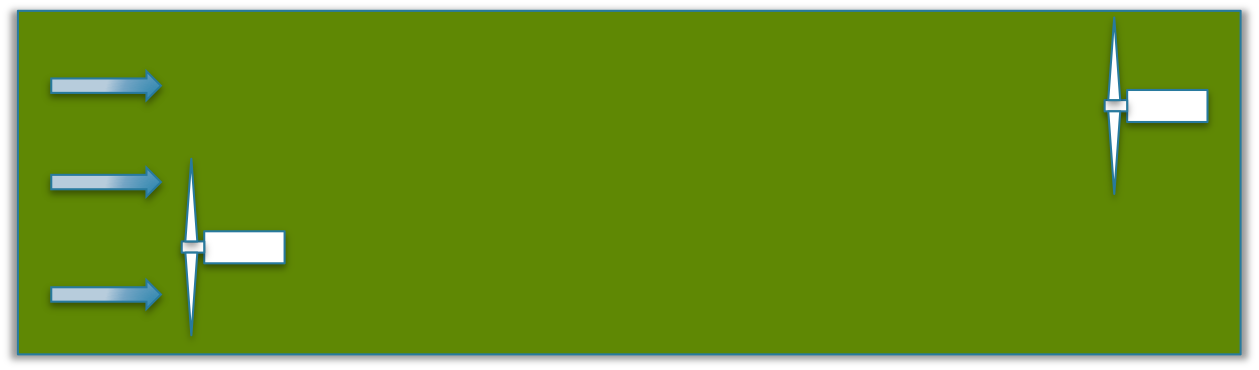
\includegraphics[width=\linewidth]{Figures/ch3Figures/fig3-5.png}
		
	\caption{Illustration of the two turbine system modeled in this chapter.}
	\label{fig3-5}
\end{figure}

Figure \ref{fig3-6} is a block diagram illustrating how FAST can be used to simulate the two turbine system shown in Figure \ref{fig3-5}. First a simulated wind field is generated. This can be a simple wind field, such as  uniform incoming wind, or a turbulent wind field generated with TurbSim. Next, FAST is used to simulate how a turbine with a conventional control system will respond to the  wind field. This first FAST simulation simulates the upwind turbine in our two turbine system. Once the first FAST simulation is complete, the simulation results are post-processed using the wind speed estimation techniques described in \ref{section2-4}. In real world applications, data from the upwind turbine would be continually processed and passed to the downwind turbine. However, since we are simulating the upwind and downwind turbine separately, it is easier to process all of the upwind turbine data at the same time. Finally, FAST is used to simulate the downwind turbine. In this second simulation the turbine experiences the same wind field, but the turbine has feed forward pitch control and has access to wind speed preview data that was generated by post processing the results of the upwind turbine simulation. By comparing the simulation results from the first (upwind) and second (downwind) FAST simulations we can see how the feed forward pitch controller has affected turbine performance.

 \begin{figure}[htbp]
	\centering
		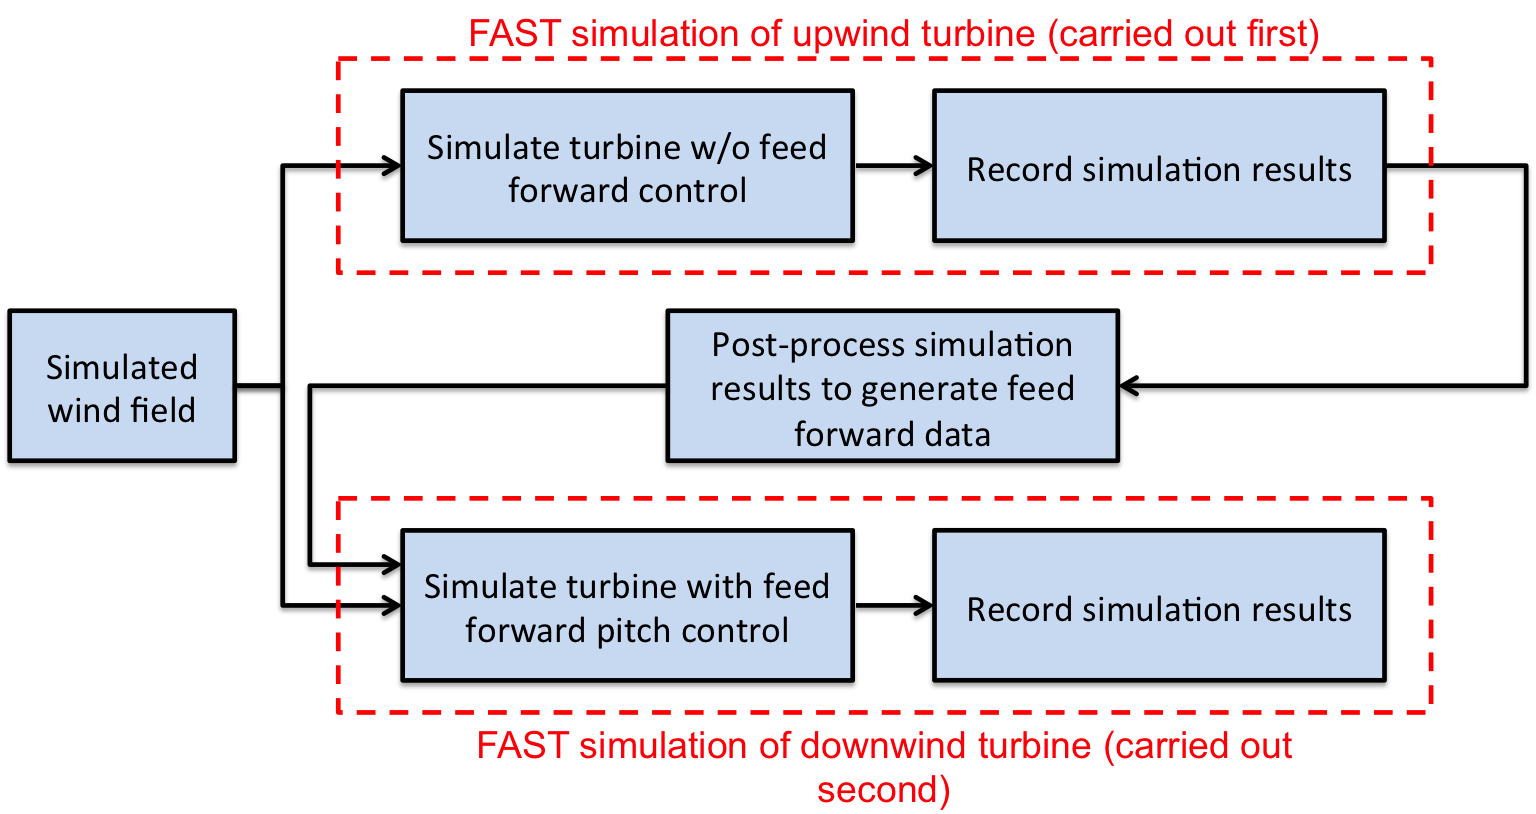
\includegraphics[width=\linewidth]{Figures/ch3Figures/fig3-6.png}
		
	\caption{The process used to simulate a two turbine system with FAST.}
	\label{fig3-6}
\end{figure}


%----------------------------------------------------------------------------------------
%	SECTION 3
%----------------------------------------------------------------------------------------

\section{Controller Design} \label{section3-3}

\subsection{Implementing Feed Forward Control} \label{section3-3-1}

Figure \ref{fig3-7} is a simple block diagram illustrating how the control system, turbine, and wind interact for a typical utility scale turbine. The behavior of the turbine is affected by the wind as well as the collective pitch ($\theta$) and generator torque ($T_{Gen}$) commands sent by the closed loop controller. The closed loop controller monitors the turbine rotor speed ($\Omega_{Rotor}$), the only feedback signal used in a typical utility scale turbine controller, to determine if the turbine is operating at a desired steady state operating point. If the turbine is not at a desired operating point the controller manipulates collective blade pitch ($\theta$) and generator torque ($T_{Gen}$) to bring the turbine to a desired operating point. In region 3 (high wind speeds) the controller tries to keep the turbine rotor speed ($\Omega_{Rotor}$) and power generation constant. In region 2 (low and medium wind speeds) the controller tries to maintain the rotor speed that will maximize power generation. From a control standpoint the wind is a disturbance, it is an uncontrolled input that affects the behavior of the turbine. Generally, changes in the wind cause the turbine to move away from desired operating points while the closed loop controller acts to bring the turbine back to desired operating points.


 \begin{figure}[htbp]
	\centering
		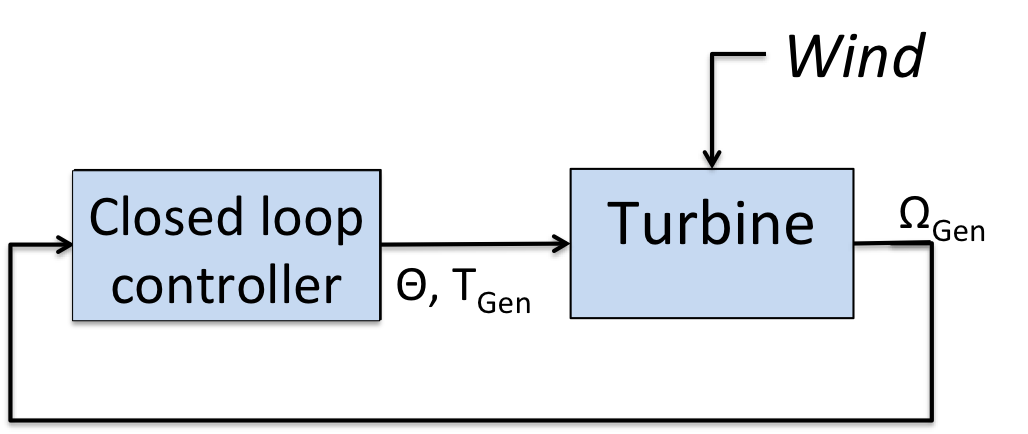
\includegraphics[width=.6\linewidth]{Figures/ch3Figures/fig3-7.png}
		
	\caption{Simple block diagram of turbine control w/o feed forward control.}
	\label{fig3-7}
\end{figure}

Figure \ref{fig3-8} is a simple block diagram illustrating the method we have chosen  to incorporate feed forward control into the control system of a turbine. You can see that the feedback control loop shown in Figure \ref{fig3-7} remains intact, but a feed forward controller, which issues supplemental collective pitch ($\theta_{ff}$) and generator torque ($T_{ff}$) commands has been added. The closed loop controller shown in Figure \ref{fig3-8} is identical to the one in Figure \ref{fig3-7}. This is not the only way to implement feed forward control, but this method does have some advantages. It is fairly simple in that it does not require us to re-design the entire control system. In addition, if the turbine were to lose the feed forward signal for any reason it would simple begin operating as if it were using a standard closed loop turbine control system. In fact this feed forward control implementation allows the turbine to smoothly transition between standard closed loop control and closed loop with feed forward control. This trait is desirable for a variety of situations. For example, if the wind changes direction the turbine may find that it no longer has an upwind turbine to use as a sensor.

 \begin{figure}[htbp]
	\centering
		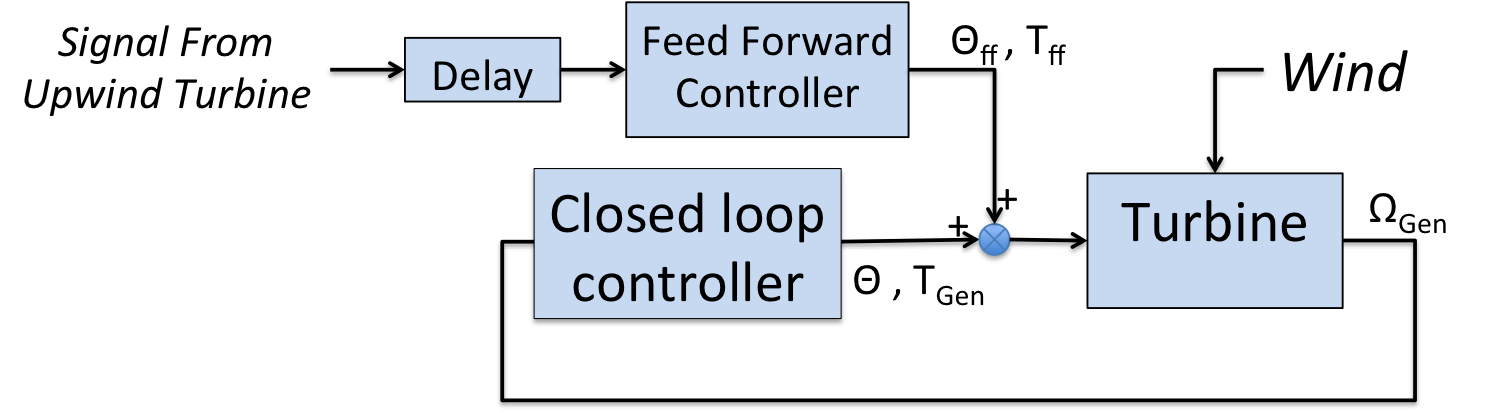
\includegraphics[width=\linewidth]{Figures/ch3Figures/fig3-8.png}
		
	\caption{Simple block diagram of turbine with feed forward control.}
	\label{fig3-8}
\end{figure}

\subsection{Closed Loop Controller}

The closed loop controller is modeled in Simulink and coupled to FAST as described in the FAST user's guide \cite{jonkman2005}, and the full Simulink model of the closed loop controller can be found in appendix \ref{AppendixB}. The controller has all the properties of the NREL 5-MW controller defined by NREL in \cite{jonkman2009} plus a model of the collective blade pitch actuator.  Figure \ref{fig3-9} illustrates the controller. The NREL 5-MW controller defined in \cite{jonkman2009} consists of a measurement filter, a torque controller, and a pitch controller. The measurement filter is a recursive, single pole low pass filter with a corner frequency of 0.25 Hz. The purpose of this low pass filter is to mitigate high frequency excitations of the control system. The torque controller uses a torque schedule, basing generator torque on the rotational speed of the turbine. The pitch controller is a non-linear PI (proportional and integral) controller where the proportional and integral gains are a function of blade pitch. 

Since this chapter is concerned with feed forward pitch control, the turbine will be operating in control region 3 for all simulations. The NREL 5-MW turbine operates in control region 3 when wind speeds are higher that the turbine's rated wind speed of 11.4 m/s. In control region 3 the pitch controller varies collective blade pitch in an attempt to maintain a constant rotational rotor speed ($\omega_{Rotor}$) of 12.1 RPM. When the rotor is spinning at 12.1 RPM the generator supplies the rated generator torque (43,093.55 Nm ), but when the rotor deviates from 12.1 RPM the torque controller varies torque in an effort to maintain a constant power generation of 5 MW. 

The controller shown in figure \ref{fig3-9} also includes a model of the collective pitch actuator. Though the pitch actuator is not part of the control system it must be modeled in Simulink because current versions of FAST do not model pitch actuator dynamics. If pitch actuator dynamics are not modeled, the closed loop controller is able to instantly change blade pitch. This is physically unrealistic and in some circumstances it leads to unrealistic control system behavior, such as high frequency fluctuations in pitch or unrealistic reactions to feed forward pitch control.

 \begin{figure}[htbp]
	\centering
		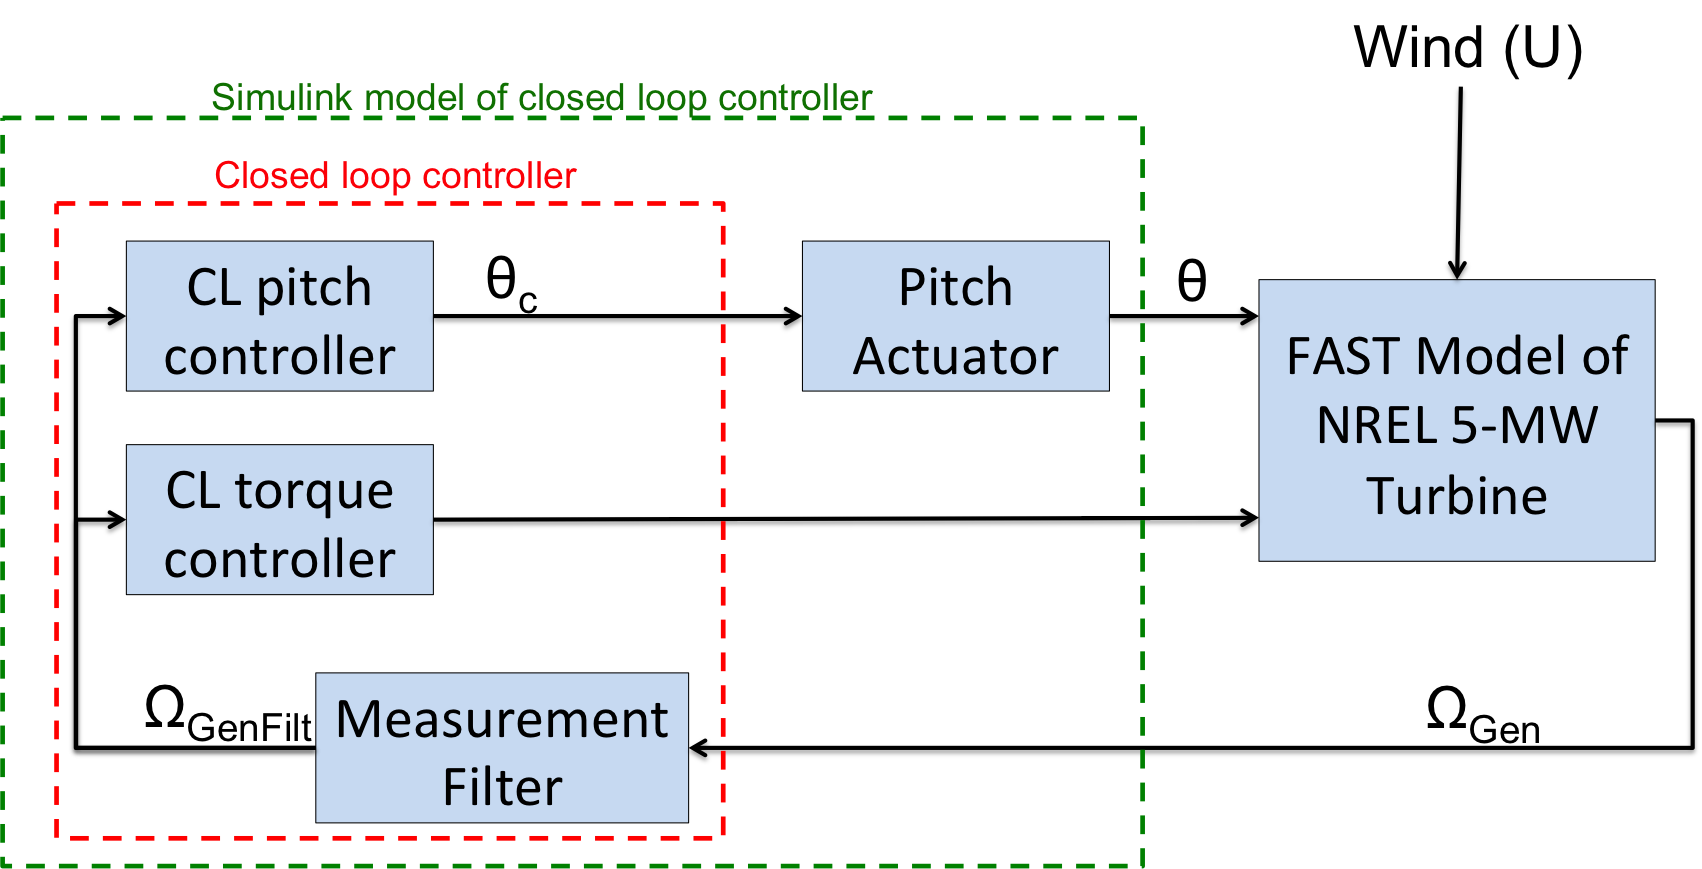
\includegraphics[width=\linewidth]{Figures/ch3Figures/fig3-9.png}
		
	\caption{Block diagram of the NREL 5-MW closed loop control system, as modeled in this dissertation.}
	\label{fig3-9}
\end{figure}

The pitch actuator is modeled as a second order system with dynamics describe by equation \ref{eq3-1}, where  $\theta$  is the actual collective blade pitch, $\theta_c$ is the desired blade pitch requested by the controller, $\xi$ is the damping ratio of the pitch actuator, and $\omega_o$ is the undamped natural frequency of the pitch actuator. Jonkman does define a NREL 5-MW blade pitch actuator in \cite{jonkman2009}, but Jonkman has admitted that the pitch actuator defined in \cite{jonkman2009} is very fast and is unrealistic \cite{jonkman2014}. Instead we use $\xi = 0.7$ and $\omega_o = 1Hz$, which have been used to model NREL 5-MW pitch actuators in previous research on feed forward turbine pitch control \cite{dunne2011,dunne2012}. 

\begin{equation}
	\ddot{\theta } + 2\xi \omega_o \dot{\theta} + \omega_{o}^{2}\theta = \omega_{o}^{2}\theta_c \label{eq3-1}
\end{equation}




\subsection{Feed Forward Controller} \label{section3-3-3}

The feed forward controller is based on the dynamic feed forward pitch controller proposed by Shlipf in \cite{schlipf2010}. Figure \ref{fig3-10} illustrates how the feed forward controller interfaces with the closed loop controller described in the previous section. As described in Section \ref{section3-3-1}, the wind is a disturbance, an uncontrolled input that affects system behavior. Typically, changes in the wind cause the turbine to deviate from the desired operating conditions while the closed loop controller acts to bring the turbine back to the desired operating conditions. Ideally we would like the feed forward controller to cancel out the effect of the disturbance so the turbine never deviates from the desired operating conditions to begin with and the closed loop controller would not need to act.

 \begin{figure}[htbp]
	\centering
		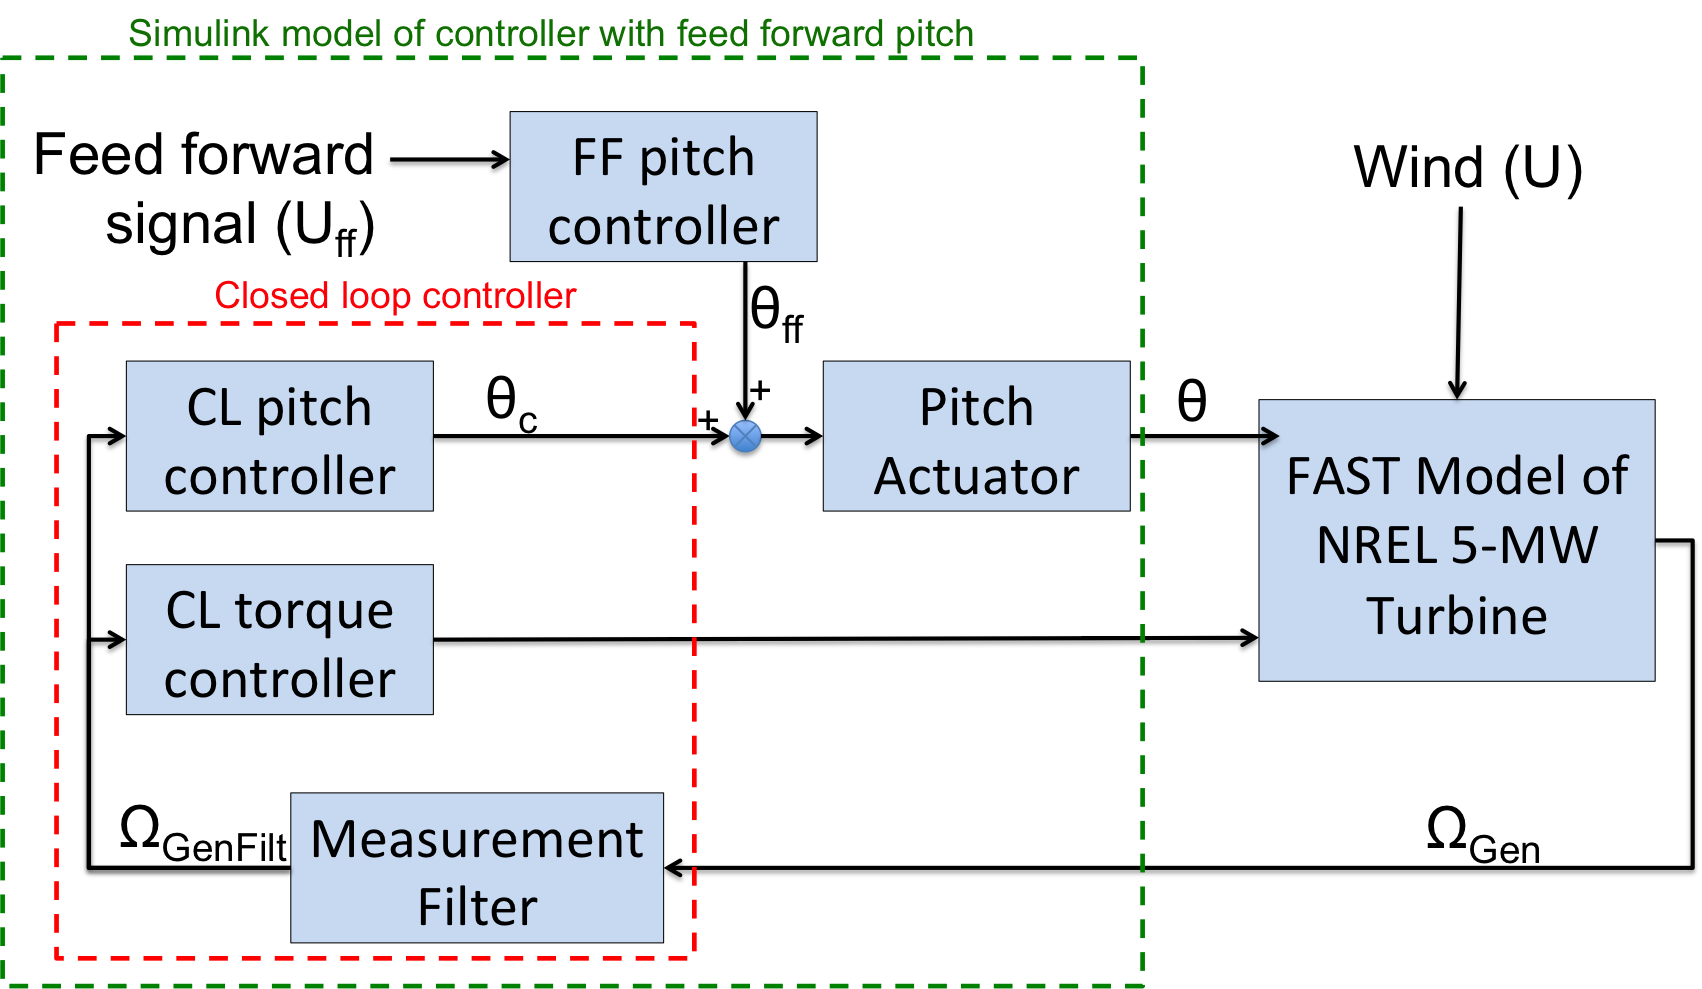
\includegraphics[width=\linewidth]{Figures/ch3Figures/fig3-10.png}
		
	\caption{Block diagram of the NREL 5-MW controller with feed forward and closed loop control.}
	\label{fig3-10}
\end{figure}

As discussed in the previous section, the goal of region 3 pitch control is to maintain a constant rotor speed of 12.1 RPM. This constant rotor speed is maintained when the aerodynamic torque applied to the rotor by the wind is equal to the torque applied to the rotor by the generator and there is no net torque to accelerate or decelerate the rotor. If the rotor is spinning at 12.1 RPM and the wind speed is anywhere between the rated wind speed (11.4 m/s) and the cutout wind speed (25 m/s) of the turbine there is a pitch angle ($\theta$) that will cause an aerodynamic torque on the rotor that perfectly matches the torque applied to the rotor by the generator. We'll call this pitch angle the steady state pitch ($\theta_{ss}$). Though the steady state pitch can't be calculated it can estimated through simulation. The relationship between steady state pitch and wind speed is shown in Figure \ref{fig3-11}.

 \begin{figure}[htbp]
	\centering
		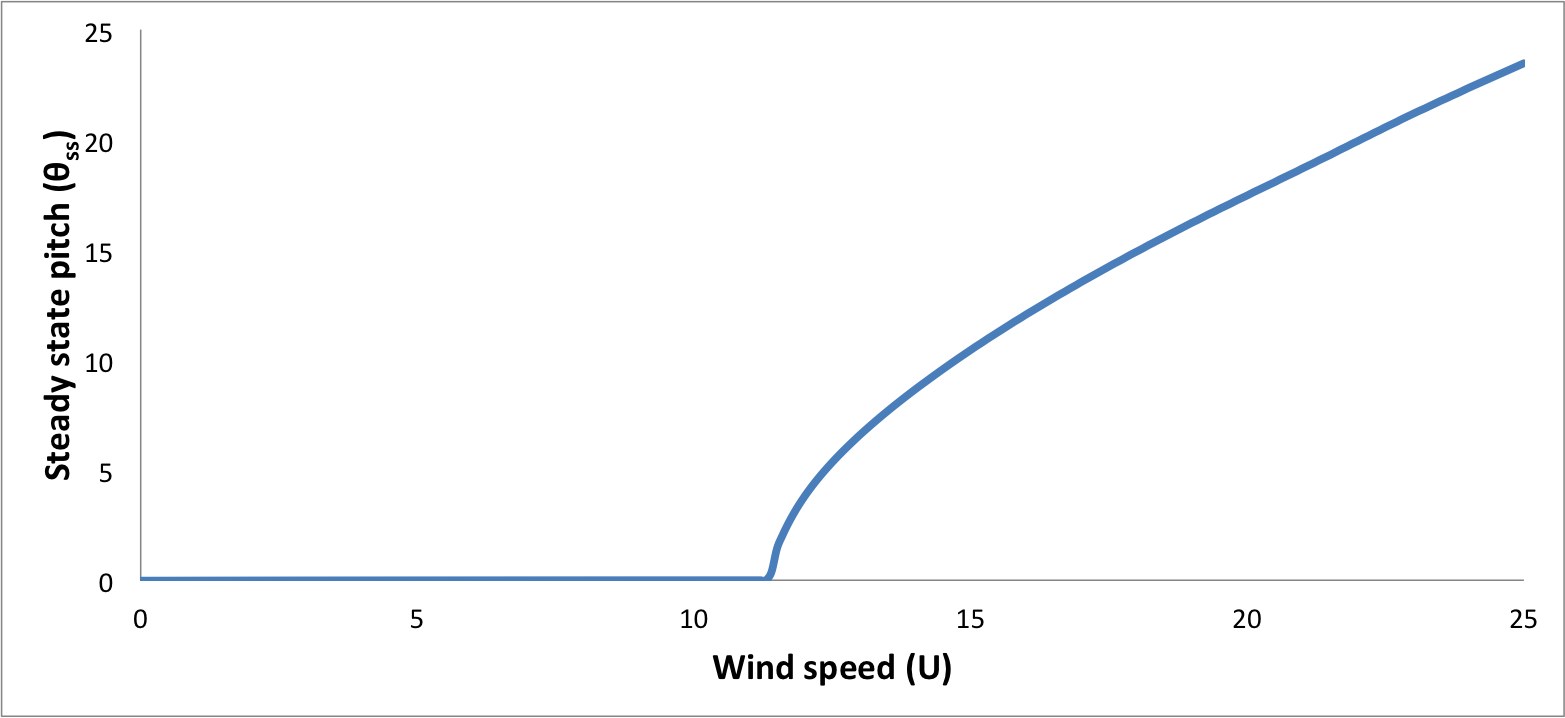
\includegraphics[width=\linewidth]{Figures/ch3Figures/fig3-11.png}
		
	\caption{Steady state pitch ($\theta_{s}$), in \degree, as a function of incoming wind speed, in m/s.}
	\label{fig3-11}
\end{figure}

If the collective blade pitch of the turbine ($\theta$) always matches the steady state pitch ($\theta_{ss}$) for the incoming wind speed ($U$) then the turbine will never deviate from the rated rotor speed of 12.1 RPM. If the feed forward signal $U_{ff}$ is an accurate estimate of the incoming wind speed (U) then it is possible to design a feed forward controller that causes the collective blade pitch to always match the corresponding steady state pitch. Since all pitch commands pass through the pitch actuators we can only ensure the correct feed forward pitch signal if we first pass the feed forward signal $U_{ff}$ through a function that inverts the dynamics of the blade pitch actuator. Therefore, the pitch commands supplied by the feed forward pitch controller ($\theta_{ff}$) is given by the equations \ref{eq3-2} and \ref{eq3-3}. $\theta_{ss}$ is the steady state pitch function that was experimentally determined and is illustrated in Figure \ref{fig3-11}. $U_{ffd}$ is the dynamic feed forward velocity, which accounts for and cancels out the dynamics of the pitch actuator.

\begin{equation}
	\theta_{ff} =  \theta_{ss}(U_{ffd}) \label{eq3-2}
\end{equation}

\begin{equation}
	U_{ffd} =  (\ddot{U} + 2 \xi \omega_o \dot{U} + \omega_o^2 U) / \omega_o^2 \label{eq3-3}
\end{equation}

If the feed forward wind speed estimate $U_{ff}$ is perfectly accurate then the feed forward signal generated using equations \ref{eq3-2} and \ref{eq3-3} will completely compensate for fluctuations in wind speed and the closed loop controller will never issue a pitch command. However, we know that in practice $U_{ff}$ will not be a perfect estimate of incoming wind speed and the closed loop controller will act whenever the feed forward pitch controller does not perfectly compensate for fluctuations in wind speed.

%----------------------------------------------------------------------------------------
%	SECTION 4
%----------------------------------------------------------------------------------------
\section{Performance With Perfect Wind Speed \\
		Knowledge} \label{section3-4}

Now that the feed forward control system has been defined the performance of this feed forward control system can be examined. In the following sections we examine the performance of the feed forward controller when it has perfect knowledge of the incoming wind speed. Two wind cases are examined. The first case is a large gust. These occur infrequently, but can be very damaging to a turbine. The second case is a turbulent wind inflow, which is typical of what a turbine experiences in day to day operation. In any real world implementation of this control system the feed forward controller will have imperfect knowledge of the incoming wind. As discussed in Chapter \ref{Chapter2}, a wind speed estimator provides imperfect estimates of both the wind speed (see Section  \ref{section2-4-1}) and convection velocity (see Section \ref{section2-5}). In addition, we know that Taylor's frozen turbulence hypothesis is not entirely accurate in practice and the wind speed fluctuations experienced by the downwind turbine will not be identical to the wind speed fluctuations experienced by the upwind turbine. However, simulating the feed forward control system with perfect knowledge of the incoming wind speed can provide valuable insight into the behavior of the feed forward control system, and can demonstrate the performance improvements that might be possible when the feed forward controller described in Section \ref{section3-3} is operated in ideal conditions. 



%----------------------------------------------------------------------------------------
%	SUBSECTION 4-1
%----------------------------------------------------------------------------------------
\subsection{Gust Response}\label{section3-4-1}

Figure \ref{fig3-12} shows an extreme operating gust for an NREL 5-MW turbine operating in 16 m/s wind according to IEC 61400-1 \cite{IEC2005}. Though extreme operating gusts occur infrequently, they can be very damaging to a wind turbine when they do occur. To examine the system's response to this extreme operating gust, both the upwind turbine and downwind turbine are subjected to a uniform wind inflow (i.e. the wind has no turbulence and all points on the turbine rotor are subjected to the same wind speed) with the magnitude shown in Figure \ref{fig3-12}. Since we are assuming the feed forward controller has perfect knowledge of the incoming wind speed, the wind speed information in Figure \ref{fig3-12} is also used as the feed forward wind speed estimate.


\begin{figure}[htbp]
	\centering
		\includegraphics[width = \linewidth]{Figures/ch3Figures/fig3-12.png}
		
	\caption{Extreme operating gust.}
	\label{fig3-12}
\end{figure}


Figures \ref{fig3-13} through \ref{fig3-17} illustrate how the upwind and downwind turbines respond to the 16 m/s extreme operating gust, while Table \ref{Table3-1} is a summary of some of the performance metrics that will be discussed in the following paragraph. By comparing the response of the upwind turbine, which does not have feed forward pitch control, to the response of the downwind turbine, which does have feed forward pith control, we can see how feed forward pitch control affects turbine performance.

In Figure \ref{fig3-13} it can be observed that the turbine with feed forward pitch control (the downwind turbine) responds to the gust sooner than the turbine without feed forward control (the upwind turbine). This is unsurprising. As discussed in Section \ref{section3-1}, a turbine using only closed loop control will respond reactively to changes in turbine behavior, which are caused by changes in wind speed. On the other hand, a turbine with feed forward control can respond to changes in wind speed before they affect turbine behavior. In fact, a perfect feed forward controller would prevent the wind speed changes from affecting turbine behavior at all. We can also see in Figure \ref{fig3-13} that the turbine with feed forward control has  higher maximum pitch angle when responding to the gust, and that the blade motion has less transient behavior after the gust passes.

\begin{figure}[htbp]
	\centering
		\includegraphics[width = \linewidth]{Figures/ch3Figures/fig3-13.png}
		
	\caption{Blade pitch response to extreme operating gust. }
	\label{fig3-13}
\end{figure}

Figure \ref{fig3-14} shows that deviations from the rated rotor speed of 12.1 RPM are greatly reduced with feed forward control. The turbine with feed forward control has a maximum rotor speed of 12.17 RPM, which is only 0.6$\%$ over the rated speed. Without feed forward control, the rotor speed reaches a peak value of 14.27 RPM, which is 17.9$\%$ over the rated rotor speed. A 17.9$\%$ rotor overspeed can be problematic as it may cause an emergency shut down of the turbine. According to Tobias Wehrhan of Oak Engineering LLC the threshold for an overspeed shut down is usually 15-20$\%$ over the rated rotor speed, depending on the turbine (personal communication, March 19, 2015). Once an overspeed shut down has been initiated, the turbine stops generating power until it can be safely restarted. This can lead to a significant loss of generated energy and therefore a loss of revenue for the turbine operator.

\begin{figure}[htbp]
	\centering
		\includegraphics[width = \linewidth]{Figures/ch3Figures/fig3-14.png}
		
	\caption{Rotor speed for turbine subjected to extreme operating gust. }
	\label{fig3-14}
\end{figure}

Figure \ref{fig3-15} shows that deviations from the rated power are greatly reduced with feed forward control. It is desirable to limit spikes in power. Power spikes can cause an emergency shut down of the turbine if it drives the DC-bus voltage above safe levels, which is typically 15-18$\%$ above the nominal DC-bus voltage (Tobias Wehrhan, personal communication, March 19, 2015). FAST does not model the DC-bus voltage, so these results don't show how close the turbine without feed forward control comes to triggering an over voltage shut-down. Table \ref{Table3-1} shows the total energy generated in each simulation. We see that the performance improvements from feed forward control are achieved without a cost to energy generation. The turbine with feed forward control actually generates slightly more power than the turbine without feed forward control.


\begin{figure}[htbp]
	\centering
		\includegraphics[width = \linewidth]{Figures/ch3Figures/fig3-15.png}
		
	\caption{Power generation for turbine subjected to extreme operating gust.}
	\label{fig3-15}
\end{figure}

Excessive structural loading can cause turbine components to immediately fail, or can cause excessive wear and tear that shortens the life of turbine components. When turbine components fail the turbine must be shut down and repaired. If we can reduce the frequency of shut downs and repairs we can increase the revenue (by increasing energy generation) and decrease the cost to the turbine operator. There are many turbine components that can experience damage from gust loading. In this section we have chosen to examine two loads, the fore-aft bending moment at the base of the tower (Figure \ref{fig3-16}) and bending moment at the root of one of the turbine blades (Figure \ref{fig3-17}). We see similar behavior in both Figures. The turbine with feed forward control experiences lower loads during the extreme operating gust, while experiencing nearly identical loads at all other times. The feed forward controller reduces the maximum tower bending moment from 100,030 kNm to 50,900 kNm, a reduction of nearly 50$\%$, and reduces the maximum blade root moment from 11,617 kNm to 7,351 kNm, a reduction of 37$\%$.

\begin{figure}[htbp]
	\centering
		\includegraphics[width = \linewidth]{Figures/ch3Figures/fig3-16.png}
		
	\caption{Tower base fore-aft moment for turbine subjected to extreme operating gust.}
	\label{fig3-16}
\end{figure}

\begin{figure}[htbp]
	\centering
		\includegraphics[width = \linewidth]{Figures/ch3Figures/fig3-17.png}
		
	\caption{Blade root bending moment for turbine subjected to extreme operating gust.}
	\label{fig3-17}
\end{figure}

Table \ref{Table3-1} summarizes the performance metrics that have been discussed in this subsection. We see that feed forward control has significantly reduced structural loading of the turbine without decreasing energy generation. This can potentially lead to a reduction in the repair and maintenance costs of the turbine without a reduction in revenue from the turbine. The turbine without feed forward control experienced a 17.9$\%$ rotor overspeed, which may be enough to induce an emergency shutdown of the turbine. Overspeed shut down faults are not modeled in theses simulations, but if the turbine without feed forward control experienced an overspeed shut down then it would generate significantly less energy than the turbine with feed forward control. In that scenario the turbine with feed forward control would have lower repair and maintenance costs while having higher revenue from energy generation.

\begin{table}
\centering
\begin{tabular}{ c | c c c c }
\hline
\hline
Turbine			& Max Tower	Base		& Max Blade	Root		& Max Rotor				& Energy\\
Control			& Bending Moment		& Bending Moment		& Overspeed					& Generated\\
					& (MNm)  				& (MNm)				& ($\%$)	& (kWh)\\
\hline
  &  &   &  &  \\
Closed Loop  & 100.00 & 11.62  &17.9 & 831.74 \\
 &  &   &  & \\
Closed Loop  &  &   &  &  \\
With Feed  & 50.90 & 7.35  & 0.6 & 831.75 \\
Forward  &  &   &  &  \\
\hline
\hline
\end{tabular}
\caption{Extreme operating gust response with perfect wind speed knowledge.}
\label{Table3-1}
\end{table}

%----------------------------------------------------------------------------------------
%	SUBSECTION 4-2
%----------------------------------------------------------------------------------------
\subsection{Turbulent Wind Response} \label{section3-4-2}

In this subsection we examine how our two turbine system reacts to turbulent wind. Like the previous subsection, both the upwind turbine and downwind turbine are subjected to the same wind speed fluctuations. The downwind turbine is equipped with the feed forward controller described in Subsection \ref{section3-3-3} and is assumed to have perfect knowledge of the incoming wind. The feed forward controller relies on knowledge of the incoming wind speed and the derivatives of the incoming wind speed. However, in a turbulent wind field the wind speed is not constant over the swept area of the rotor so there is no single measurement that can be considered the true incoming wind speed. In this subsection we will treat the average wind speed over the swept area of the rotor as the wind speed. Because this rotor average wind speed has some high frequency fluctuations it is passed through a single pole low-pass filter with a corner frequency of 0.5 Hz to generate the feed forward wind speed.

Figure \ref{fig3-18} shows the rotor average wind speed and feed forward wind speed for 200 seconds of the turbulent wind field used in this subsection. The complete wind field is 600 seconds long and was generated by TurbSim using a 16 m/s mean wind speed and the GPLLJ turbulence model. This was one of the 66 test cases used in Chapter \ref{Chapter2} and more details about this test case can be found in Section \ref{section2-2}. Figures \ref{fig3-19} through \ref{fig3-23} illustrate how the upwind and downwind turbines respond to the turbulent wind field. All figures in this subsection have the same axes as the corresponding figures in Subsection \ref{section3-4-1}. This helps illustrate the differences in magnitude between the wind turbine response to an extreme operating gust and the wind turbine response to a turbulent wind field with the same mean wind speed.

\begin{figure}[htbp]
	\centering
		\includegraphics[width = \linewidth]{Figures/ch3Figures/fig3-18.png}
		
	\caption{Rotor average wind speed and feed forward wind speed for 16 m/s turbulent wind.}
	\label{fig3-18}
\end{figure}

In Figure \ref{fig3-19} we see the blade pitch response of each turbine. We see that the blade pitch response of each turbine follows a similar pattern of peaks and valleys. However, for the turbine with feed forward pitch control the peaks and valleys occurs a few seconds earlier. This is expected because both turbines are reacting to the same fluctuations in wind speed but the turbine with feed forward control can react to those wind speed fluctuations before they affect turbine behavior. 

\begin{figure}[htbp]
	\centering
		\includegraphics[width = \linewidth]{Figures/ch3Figures/fig3-19.png}
		
	\caption{Blade pitch response to 16 m/s turbulent wind.}
	\label{fig3-19}
\end{figure}

Figures \ref{fig3-20} and \ref{fig3-2} show that the feed forward controller  reduces deviations in both rotor speed and power. With feed forward control the rotor speed stays within ???$\%$ of the rated rotor speed and the power stays within ???$\%$ of the rated power. Without feed forward control the rotor speed deviates as much as ???$\%$ from the rated speed and the power deviates as much as ???$\%$ from the rated power. Though the turbine with feed forward control performs better than the turbine without feed forward control it is important to note that neither turbine has a spike in rotor speed or power that could trigger an emergency shut down.

\begin{figure}[htbp]
	\centering
		\includegraphics[width = \linewidth]{Figures/ch3Figures/fig3-20.png}
		
	\caption{Rotor speed for turbine in 16 m/s turbulent wind.}
	\label{fig3-20}
\end{figure}

\begin{figure}[htbp]
	\centering
		\includegraphics[width = \linewidth]{Figures/ch3Figures/fig3-21.png}
		
	\caption{Power generation for turbine in 16 m/s turbulent wind.}
	\label{fig3-21}
\end{figure}

Figures \ref{fig3-22} and \ref{fig3-23} show the tower fore-aft bending moment and the blade root bending moment. In the previous subsection, when we examined the turbines' responses to an extreme operating gust, it was immediately obvious that feed forward control significantly reduced loads. In figures \ref{fig3-22} and \ref{fig3-23} it is not obvious that feed forward control is reducing loads. Though there are many moments in the simulation when feed forward control reduces loading, there are also many times when feed forward control causes higher loading. To determine which control system has better performance we must statistically analyze the loading.

In the previous subsection we analyzed loading by measuring and comparing the maximum loads experienced by the turbines. For these simulation results comparing the maximum loads doesn't make sense. In the previous subsection the turbine experienced a single large spike in loading when the extreme operating gust hit the turbines. In this subsection the turbine experiences many loading cycles that all have similar amplitudes. 


\begin{figure}[htbp]
	\centering
		\includegraphics[width = \linewidth]{Figures/ch3Figures/fig3-22.png}
		
	\caption{Tower base fore-aft moment for turbine in 16 m/s turbulent wind.}
	\label{fig3-22}
\end{figure}

\begin{figure}[htbp]
	\centering
		\includegraphics[width = \linewidth]{Figures/ch3Figures/fig3-23.png}
		
	\caption{Blade root bending moment for turbine in 16 m/s turbulent wind.}
	\label{fig3-23}
\end{figure}

Table \ref{Table3-2} shows the mean and standard deviation of several turbine performance metrics. We see that feed forward control does not affect the mean values, but does decrease the variability of the performance metrics. Feed forward control reduces the standard deviation of the power by more than 50$\%$. 

Reduced variability in power generation can be beneficial for grid integration of wind turbines. The standard deviation of the tower base bending moment and the blade root bending moment are reduces by 26$\%$ and 2$\%$ respectively. 

\begin{table}
\centering
\begin{tabular}{ c | c c c c c c c c c c c c}
\hline
\hline
	& & \multicolumn{2}{c}{Tower base}	& & \multicolumn{2}{c}{Blade root}		& & \\
	& & \multicolumn{2}{c}{bending}	& & \multicolumn{2}{c}{bending}		& &\multicolumn{2}{c}{Rotor}	& & \\
	& & \multicolumn{2}{c}{moment}	& & \multicolumn{2}{c}{moment}		& &\multicolumn{2}{c}{speed}		& &\multicolumn{2}{c}{Power} \\	
Turbine					& & \multicolumn{2}{c}{(MNm)}  					& & \multicolumn{2}{c}{(MNm)}	& & \multicolumn{2}{c}{(RPM)}	& & \multicolumn{2}{c}{(kW)}\\
\cline{3-4} \cline{6-7} \cline{9-10} \cline{12-13} 
Control & & mean & $\sigma$ & & mean & $\sigma$ & & mean & $\sigma$  & & mean & $\sigma$ \\
\hline
\\
Closed loop & & 36.60 & 4.64  & & 5.96 & 1.84  && 12.0 & 0.212&& 5,000  & 21.8 \\
 \\
Closed loop \\
with feed   & & 36.60 & 3.42  & & 5.95 & 1.80 && 12.0 & 0.0547  && 5,000  & 10.7 \\
forward\\
\hline
\hline
\end{tabular}
\caption{Statistical summary of turbine performance in 16 m/s wind.}
\label{Table3-2}
\end{table}


Though a reduction in the standard deviation of the structural loads is noteworthy, it is more important to understand how the changes in structural loads will affect the wear and tear on turbine components. To estimate the wear and tear inflicted on the tower base and the blade root we can calculate the short term damage equivalent loads (DEL). An explanation of damage equivalent loads and how they were calculated in this dissertation can be found in Appendix \ref{AppendixC}. 

Table shows that for this 10 minute simulation of 16 m/s turbulent wind feed forward control reduces the damage equivalent loads for both tower base bending moment and blade root bending moment. This indicates that the turbine with feed forward control experiences less wear and tear on it's components, which may lead to less repair and maintenance costs over the life of the turbine.


\begin{table}
\centering
\begin{tabular}{ c | c c c c c c c c c}
\hline
\hline
					&&\multicolumn{2}{c}{Tower Base}					&&\multicolumn{2}{c}{Blade	Root} \\
					&&\multicolumn{2}{c}{Bending Moment}			&&\multicolumn{2}{c}{bending Moment}\\
						\cline{3-4} 														\cline{6-7}
Turbine			&& DEL   	& Change										&& DEL  	& Change\\
Control			&& (MNm)  & in DEL 										&& (MNm)  & in DEL 	\\
\hline
\\
Closed Loop  && 44.20 & - 													&& 10.58 & - \\
 \\
Closed Loop\\
With Feed  		&& 35.60 & -19.5$\%$ 									&& 10.02 & -5.3$\%$\\
Forward\\
\hline
\hline
\end{tabular}
\caption{Short term damage equivalent loads for 570 s simulation of turbine  in 16 m/s turbulent wind.}
\label{Table3-3}
\end{table}


%----------------------------------------------------------------------------------------
%	SECTION 5
%----------------------------------------------------------------------------------------
\section{Performance With Wind Speed Estimate From Upwind Turbine} \label{section3-5}
The previous sections demonstrated how the feed forward pitch controller affects performance when it has perfect knowledge of the incoming wind. However, in practice the feed forward controller will not have perfect knowledge of the incoming wind. The feed forward controller will have an estimate of the incoming wind that is generated by using the upwind turbine as a sensor. In the following subsections we examine the performance of the feed forward controller when it has only an estimate of the incoming wind speed. The incoming wind speed estimate is based on the dynamic behavior of the upwind turbine and is generated using the process described in Section \ref{section2-4}. The simulations described below assume Taylor's frozen turbulence, and assume that we will be able to perfectly determine the convection velocity. We know that neither of those assumptions will be entirely accurate in practice, but the simulations described in this section bring us a step closer to a realistic implementation of feed forward pitch control than the simulations described in the previous section.

%----------------------------------------------------------------------------------------
%	SUBSECTION 5-1
%----------------------------------------------------------------------------------------
\subsection{Gust Response} \label{section3-5-1}
Figure \ref{fig3-24} shows an extreme operating gust for an NREL 5-MW turbine operating in 16 m/s wind according to IEC 61400-1 \cite{IEC2005} and the feed forward wind speed estimate generated by the upwind turbine. This is the same extreme operating gust simulated in Section \ref{section3-4-1}. The feed forward wind speed estimate does not perfectly capture the fluctuations in wind speed. In particular, the feed forward wind speed estimate has smaller peaks and valleys and contains some transient behavior after the extreme operating gust has passed.



\begin{figure}[htbp]
	\centering
		\includegraphics[width = \linewidth]{Figures/ch3Figures/fig3-24.png}
		
	\caption{Extreme operating gust and feed forward wind speed estimate based on gust.}
	\label{fig3-24}
\end{figure}

Figure \ref{fig3-25} shows the pitch response of the turbines. As we saw in previous simulations, the turbine with feed forward pitch control reacts to the extreme operating gust sooner than the turbine without feed forward pitch control. One noteworthy feature is the large dip in blade pitch for the turbine with feed forward pitch control. The blade pitch briefly drops to 5.4$^\circ$ at approximately 110 seconds. This is potentially dangerous behavior for the turbine with feed forward pitch control. For a given wind speed, decreasing the blade pitch results in an increase in the wind energy captured by the rotor. This leads to increased structural loads and increased rotor speed. If the blade pitch suddenly drops too low, as may be the case here, it can potentially lead to spikes in structural loads or rotor speed. 

\begin{figure}[htbp]
	\centering
		\includegraphics[width = \linewidth]{Figures/ch3Figures/fig3-25.png}
		
	\caption{Blade pitch response to extreme operating gust. }
	\label{fig3-25}
\end{figure}

Figure \ref{fig3-26} shows that feed forward control significantly reduces deviations from the rated rotor speed of 12 RPM. The turbine without feed forward pitch control has a maximum rotor speed 17.9$\%$ above the rated speed. As discussed before, an overspeed of this magnitude could cause an emergency shutdown of the turbine. The turbine with feed forward pitch control has a maximum rotor speed 5.5$\%$ above the rated speed. For the turbine without feed forward control the maximum rotor speed occurs immediately after the peak of the extreme operating gust. The turbine with feed forward pitch control also has a rotor overspeed immediately after the peak of the extreme operating gust, but the maximum rotor speed occurs approximately 10 seconds later, immediately after the sudden dip in blade pitch that was observed in Figure \ref{fig3-25}. This suggests that the larges rotor overspeed experienced turbine with feed forward pitch control was caused by the control action of the feed forward controller and not by the extreme operating gust.

\begin{figure}[htbp]
	\centering
		\includegraphics[width = \linewidth]{Figures/ch3Figures/fig3-26.png}
		
	\caption{Rotor speed for turbine subjected to extreme operating gust. }
	\label{fig3-26}
\end{figure}

In the remaining figures we see similar behavior to what we see in Figure \ref{fig3-27}. Feed forward pitch control improves performance by reducing deviations from rated power (Figure \ref{fig3-27}), maximum tower fore-aft bending moments (Figure \ref{fig3-28}), and maximum blade root bending moments (Figure \ref{fig3-29}). The turbine with feed forward pitch control experiences a peak in power production and structural loads immediately after the peak of the extreme operating gust. The turbine with feed forward pitch control then experiences an even larger peak in power production and structural loads immediately after the sudden dip in blade pitch that was observed in Figure \ref{fig3-25}.

\begin{figure}[htbp]
	\centering
		\includegraphics[width = \linewidth]{Figures/ch3Figures/fig3-27.png}
		
	\caption{Power generation for turbine subjected to extreme operating gust.}
	\label{fig3-27}
\end{figure}

\begin{figure}[htbp]
	\centering
		\includegraphics[width = \linewidth]{Figures/ch3Figures/fig3-28.png}
		
	\caption{Tower base fore-aft moment for turbine subjected to extreme operating gust.}
	\label{fig3-28}
\end{figure}

\begin{figure}[htbp]
	\centering
		\includegraphics[width = \linewidth]{Figures/ch3Figures/fig3-29.png}
		
	\caption{Blade root bending moment for turbine subjected to extreme operating gust.}
	\label{fig3-29}
\end{figure}

Table \ref{Table3-4} summarizes the performance metrics for this simulation. We see that feed forward pitch control reduces structural loading of the turbine and deviations from the rated rotor speed. The use of feed forward pitch control does decrease energy capture by 0.54 kWh, but this is a very small decrease. If the wind plant sells energy for 8 cents per kWh the use of feed forward pitch control would result in a 4 cent decrease in revenue. Though feed forward pitch control does improve the turbine performance in this simulation, it is also worth noting that the feed forward pitch controller used in this simulation does not perform as well as a feed forward pitch controller with perfect knowledge of incoming wind speed (Table \ref{Table3-1}).

\begin{table}
\centering
\begin{tabular}{ c | c c c c }
\hline
\hline
Turbine			& Max Tower	Base		& Max Blade	Root		& Max Rotor				& Energy\\
Control			& Bending Moment		& Bending Moment		& Overspeed					& Generated\\
						& (MNm)  				& (MNm)				& ($\%$)	& (kWh)\\

\hline
  &  &   &  &  \\
Closed Loop  & 100.03 & 11.62  &17.9 & 831.74 \\
 &  &   &  & \\
Closed Loop  &  &   &  &  \\
With Feed  & 77.70 & 10.51  & 5.5 & 831.20 \\
Forward  &  &   &  &  \\
\hline
\hline
\end{tabular}
\caption{EOG response with feed forward signal based on wind speed estimate.}
\label{Table3-4}
\end{table}

%----------------------------------------------------------------------------------------
%	SUBSECTION 5-2
%----------------------------------------------------------------------------------------
\subsection{Turbulent Wind Response} \label{section3-5-2}
Figure \ref{fig3-30} shows the rotor average wind speed and feed forward wind speed for 200 seconds of the turbulent wind field used in this subsection. This subsection uses the same turbulent wind field used in Subsection \ref{section3-4-2}. Though the feed forward wind speed, estimated through the rotor dynamics of the upwind turbine, does not perfectly match the rotor average wind speed, it does capture most of the peaks and valleys of the wind speed fluctuations. 

\begin{figure}[htbp]
	\centering
		\includegraphics[width = \linewidth]{Figures/ch3Figures/fig3-30.png}
		
	\caption{Rotor average wind speed and feed forward wind speed estimate of turbulent 16 m/s wind.}
	\label{fig3-30}
\end{figure}

Figures \ref{fig3-31} through \ref{fig3-35} show the dynamic behavior of a turbine with and without feed forward pitch control. We see in these figures that feed forward control reduces deviations in blade pitch (Figure \ref{fig3-31}), rotor speed (Figure \ref{fig3-32}), and power production (Figure \ref{fig3-33}). However, feed forward control does not reduce these deviations as much as we saw when the feed forward wind speed was the true rotor average wind speed (Subsection \ref{section3-4-2}). 

\begin{figure}[htbp]
	\centering
		\includegraphics[width = \linewidth]{Figures/ch3Figures/fig3-31.png}
		
	\caption{Blade pitch response to 16 m/s turbulent wind.}
	\label{fig3-31}
\end{figure}

\begin{figure}[htbp]
	\centering
		\includegraphics[width = \linewidth]{Figures/ch3Figures/fig3-32.png}
		
	\caption{Rotor speed for turbine in 16 m/s turbulent wind.}
	\label{fig3-32}
\end{figure}

\begin{figure}[htbp]
	\centering
		\includegraphics[width = \linewidth]{Figures/ch3Figures/fig3-33.png}
		
	\caption{Power generation for turbine in 16 m/s turbulent wind.}
	\label{fig3-33}
\end{figure}

In Figures \ref{fig3-34} and \ref{fig3-35} it is difficult to determine how feed forward control affects the structural loading of the turbine components. However, Table \ref{Table3-6} shows that feed forward control does in fact reduce the damage equivalent loads of the tower base bending moment (11.8$\%$ reduction) and the blade root bending moment (5.7$\%$ reduction). Note that these reductions in damage equivalent loads are not as large as the reductions observed when the feed forward wind speed was the true rotor average wind speed (Subsection \ref{section3-4-2}). 

\begin{figure}[htbp]
	\centering
		\includegraphics[width = \linewidth]{Figures/ch3Figures/fig3-34.png}
		
	\caption{Tower base fore-aft moment for turbine in 16 m/s turbulent wind.}
	\label{fig3-34}
\end{figure}

\begin{figure}[htbp]
	\centering
		\includegraphics[width = \linewidth]{Figures/ch3Figures/fig3-35.png}
		
	\caption{Blade root bending moment for turbine in 16 m/s turbulent wind.}
	\label{fig3-35}
\end{figure}


\begin{table}
\centering
\begin{tabular}{ c | c c c c c c c c c c c c}
\hline
\hline
	& & \multicolumn{2}{c}{Tower Base}	& & \multicolumn{2}{c}{Blade Root}		& & \\
	& & \multicolumn{2}{c}{Bending}	& & \multicolumn{2}{c}{Bending}		& &\multicolumn{2}{c}{Rotor}	& & \\
	& & \multicolumn{2}{c}{Moment}	& & \multicolumn{2}{c}{Moment}		& &\multicolumn{2}{c}{Speed}		& &\multicolumn{2}{c}{Power} \\	
Turbine					& & \multicolumn{2}{c}{(MNm)}  					& & \multicolumn{2}{c}{(MNm)}	& & \multicolumn{2}{c}{(RPM)}	& & \multicolumn{2}{c}{(kW)}\\
\cline{3-4} \cline{6-7} \cline{9-10} \cline{12-13} 
Control & & mean & $\sigma$ & & mean & $\sigma$ & & mean & $\sigma$  & & mean & $\sigma$ \\
\hline
\\
Closed Loop  & & 36.60 & 4.64  & & 5.96 & 1.84  && 12.0 & 0.212&& 5,000  & 21.8 \\
 \\
Closed Loop\\
With Feed  & & 36.50 & 3.60  & & 5.95 & 1.79 && 12.0 & 0.081  && 5,000  & 12.0 \\
Forward\\
\hline
\hline
\end{tabular}
\caption{Statistical summary of turbine performance in 16 m/s wind.}
\label{Table3-5}
\end{table}

\begin{table}
\centering
\begin{tabular}{ c | c c c c c c c c c}
\hline
\hline
					&&\multicolumn{2}{c}{Tower Base}					&&\multicolumn{2}{c}{Blade	Root} \\
					&&\multicolumn{2}{c}{Bending Moment}			&&\multicolumn{2}{c}{Bending Moment}\\
						\cline{3-4} 														\cline{6-7}
Turbine			&& DEL   	& Change										&& DEL  	& Change\\
Control			&& (MNm)  & in DEL 										&& (MNm)  & in DEL 	\\
\hline
\\
Closed Loop  && 44.20 & - 													&& 10.58 & - \\
 \\
Closed Loop\\
With Feed  		&& 39.00 & -11.8$\%$ 									&& 9.98 & -5.7$\%$\\
Forward\\
\hline
\hline
\end{tabular}
\caption{Short term damage equivalent loads for 570 s simulation of turbine  in 16 m/s turbulent wind.}
\label{Table3-6}
\end{table}

%----------------------------------------------------------------------------------------
%	SECTION 6
%----------------------------------------------------------------------------------------

\section{Sensitivity to Errors in Feed Forward Data \\
		Timing}  \label{section3-6}
In the previous section we observed that feed forward pitch control based on wind speed estimates from an upwind turbine can improve performance and reduce structural loading provided Taylor's frozen turbulence holds and we are able to perfectly estimate the convection speed of the wind. However, experiments have shown that Taylor's frozen turbulence hypothesis is never completely accurate and it is impossible to perfectly estimate the convection velocity. In this section we bring our system one step closer to reality by considering the effect of errors in the convection velocity estimate.

In Section \ref{section2-5} we discussed a method for estimating the convection velocity by calculating the mean wind speed estimate over some period of time. For the 66 test cases examined in Section \ref{section2-5} we found that the accuracy of the convection velocity estimate varied with both the true mean wind speed, and the time period over which the wind speed estimates were averaged. For wind speeds above the rated wind speed (the conditions we are considering for feed forward pitch control) the mean discrepancy between the true and estimated convection velocity ranged from ~2$\%$ to ~4$\%$.

By making a few reasonable assumptions about our system, we can get a rough estimate of the convection velocity error we might expect for the 16 m$/$s turbulent wind field our system was subjected to in sections \ref{section3-4-2} and \ref{section3-5-2}. We can also determine how that convection velocity error would affect the timing of the feed forward wind speed estimates received by the downwind turbine. If we assume a 60 second averaging time, we might expect the error in our convection velocity estimate to average approximately 3.2$\%$ (Figure \ref{fig3-26}), or 0.5 m/s. If we assume the downwind turbine is 10 rotor diameters, or 1260 meters, behind the upwind turbine a 3.2$\%$ error in the convection velocity estimate will cause an error in the timing of the feed forward of approximately 2.5 seconds.

We can simulate the effect of an error in the convection velocity estimate by modifying the turbulent wind response simulation from Section \ref{section3-5-2}. Instead of using perfectly timed feed forward wind speed estimates, the feed forward wind speed estimates is shifted in time. To determine how errors in the convection velocity estimate affect system performance we can calculate the resulting damage equivalent loads (DEL) on the tower bending moment and blade root moment.

Figure \ref{fig3-36} illustrates how timing errors in the feed forward data affect the damage equivalent load of the tower fore-aft bending moment. A negative timing error indicates the feed forward data is ahead of the turbulent wind field. In other words, the system has overestimated the convection velocity and as a result the turbulent wind fluctuations are arriving at the downwind turbine later than the system expects them to. 

The red line indicates the tower base DEL for the upwind turbine. Since the upwind turbine does not depend on feed forward data, the tower base DEL for the upwind turbine is constant across all simulations. The blue line indicates the tower base DEL for the downwind turbine. We see from the figure that a small negative error in the convection velocity estimate actually improves performance. The minimum damage equivalent load corresponds to a timing error of approximately -0.5 seconds. We also see that if the timing error is less than -2.2 seconds or greater than 0.8 seconds the turbine with feed forward control performs worse that the turbine without feed forward control. This is troubling because earlier in this section we estimated that our timing error for this wind speed would be in the neighborhood of $\pm$2.5 seconds.

\begin{figure}[htbp]
	\centering
		\includegraphics[width = \linewidth]{Figures/ch3Figures/fig3-35.png}
		
	\caption{Tower base DEL for various timing errors in feed forward wind speed estimates.}
	\label{fig3-36}
\end{figure}

Figure \ref{fig3-37} illustrates how timing errors in the feed forward data affect the damage equivalent load of the blade root bending moment. Again, a negative timing error indicates the feed forward data is ahead of the turbulent wind field, the red line indicates the DEL of the upwind turbine, and the blue line indicates the DEL of he downwind turbine. We see that a small negative error improves performance. Like the tower base DEL, the blade root DEL is smallest when the timing error is -0.5 seconds. We also see that if the timing error is less than -4.8 seconds or greater than 2.3 seconds the turbine with feed forward control performs worse that the turbine without feed forward control. Blade root DEL is improved over a wider range of timing errors than we saw for tower base DEL, however our estimated timing error of $\pm$2.5 seconds would not guarantee that the downwind turbine with feed forward pitch control would perform better than a turbine with conventional closed loop control.


\begin{figure}[htbp]
	\centering
		\includegraphics[width = \linewidth]{Figures/ch3Figures/fig3-35.png}
		
	\caption{Blade root DEL for various timing errors in feed forward wind speed estimates.}
	\label{fig3-37}
\end{figure}

Timing errors do not affect the average power production. Each simulations simulation had an average power production of 5,000 kW. However, timing errors do affect the standard deviation of the power production. As shown in Figure \ref{fig3-38}, feed forward pitch control reduces the standard deviation of the power production when the timing error is small, but feed forward control increases the standard deviation of the power production for timing errors greater than +2.2 seconds or less than -3.1 seconds. A small standard deviation is desirable as it indicates the power output of the turbine remains closer to the desired power output.

\begin{figure}[htbp]
	\centering
		\includegraphics[width = \linewidth]{Figures/ch3Figures/fig3-35.png}
		
	\caption{Standard deviation of power production for various timing errors in feed forward wind speed estimates.}
	\label{fig3-38}
\end{figure}

All of the data presented in this section tell the same story. The feed forward pitch control system is sensitive to timing errors. Though the feed forward control system improves performance when timing errors are small it can degrade performance when significantly large timing errors are present. Based on the convection velocity estimate study carried out in Section \ref{section2-5}, we can not guarantee timing errors will be small enough to ensure feed forward control will improve turbine performance. A control system that is just as likely to degrade performance as improve it is not particularly useful. As such, the results in this section show that in practice the proposed feed forward pitch control scheme proposed in this chapter is not very practical. At this point it is not worthwhile to carry out additional investigations into other real world complications the system would face, such as inaccuracies of the Taylor's frozen turbulence hypothesis.

%----------------------------------------------------------------------------------------
%	SECTION 7
%----------------------------------------------------------------------------------------
\section{Summary and Conclusions}

In this chapter a feed forward optimal pitch control scheme is introduced and investigated. In this control scheme an upwind is used as a wind speed sensor. Wind speed measurements are passed from the upwind turbine to a feed forward controller on a downwind turbine. These wind speed measurements give the feed forward controller information about the wind speed fluctuations the downwind turbine will experience in the future. The feed forward controller determines the optimal pitch corresponding to the incoming wind speed fluctuations and issues supplementary pitch commands to the existing feedback control loop of the downwind turbine. These supplementary pitch commands enable the downwind turbine to preemptively respond to incoming wind speed fluctuations potentially improving energy capture and reducing damage to the turbine.

The control scheme is investigated through three rounds of simulation using the NREL FAST turbine simulation tool. The initial round of simulations uses a simplified idealistic model of the system, while the subsequent rounds systematically incorporate complicating factors that a real world system would encounter.  

The first round of simulations (Section \ref{section3-4}) assumes that the feed forward controller has perfect measurements of the incoming wind speed fluctuations, that the convection velocity has been estimated perfectly, and that the wind speed fluctuations experienced by the downwind turbine will be identical to the wind speed fluctuations experienced by the upwind turbine. Results show that in these conditions feed forward control significantly improves turbine performance with respect to both extreme operating gusts and turbulent wind.

The second round of simulations assumes that the convection velocity has been estimated perfectly, and that the wind speed fluctuations experienced by the downwind turbine will be identical to the wind speed fluctuations experienced by the upwind turbine. It does not assume that the feed forward controller has perfect measurements of the incoming wind speed fluctuations. Instead, the wind speed fluctuations are estimated using the dynamics of the upwind turbine. The results from the second round of simulations show smaller performance improvements from the use of feed forward optimal pitch control (compared to the first round of simulations). However, in these conditions feed forward control still significantly improves turbine performance.

The third round of simulations assume that the wind speed fluctuations experienced by the downwind turbine will be identical to the wind speed fluctuations experienced by the upwind turbine. Wind speed fluctuations are estimated using the dynamics of the upwind turbine and a variety of timing errors are introduced to simulate the effect of errors in estimating the convection velocity. Results from this round of simulations show that the feed forward optimal pitch control system is very sensitive to timing errors. If the timing of the data is off by more than a few seconds the feed forward control system can cause a turbine to perform more poorly than a turbine without feed forward control.

The feed forward optimal pitch control scheme presented in this chapter seemed promising trough the first two rounds of simulations. However, the system's high sensitivity to timing errors, and therefore the systems high sensitivity to errors in the estimation of the convection velocity, ultimately make this control scheme impractical in real world applications. In order to effectively use an upwind turbine as a sensor to improve the performance of a downwind turbine we must investigate alternate control schemes that will be less sensitive to timing errors.
